% This is a Basic Assignment Paper but with like Code and stuff allowed in it. 

\documentclass[11pt]{article}

% Preamble

\usepackage[margin=1in]{geometry}
\usepackage{amsfonts, amsmath, amssymb}
\usepackage{fancyhdr, float, graphicx}
\usepackage[utf8]{inputenc} % Required for inputting international characters
\usepackage[T1]{fontenc} % Output font encoding for international characters
\usepackage{fouriernc} % Use the New Century Schoolbook font
\usepackage[nottoc, notlot, notlof]{tocbibind}
\usepackage{listings}
\usepackage{xcolor}

\definecolor{codegreen}{rgb}{0,0.6,0}
\definecolor{codegray}{rgb}{0.5,0.5,0.5}
\definecolor{codepurple}{rgb}{0.58,0,0.82}
\definecolor{backcolour}{rgb}{0.95,0.95,0.92}

\lstdefinestyle{mystyle}{
    backgroundcolor=\color{backcolour},   
    commentstyle=\color{codegreen},
    keywordstyle=\color{magenta},
    numberstyle=\tiny\color{codegray},
    stringstyle=\color{codepurple},
    basicstyle=\ttfamily\footnotesize,
    breakatwhitespace=false,         
    breaklines=true,                 
    captionpos=b,                    
    keepspaces=true,                 
    numbers=left,                    
    numbersep=5pt,                  
    showspaces=false,                
    showstringspaces=false,
    showtabs=false,                  
    tabsize=2
}

\lstset{style=mystyle}

% Header and Footer
\pagestyle{fancy}
\fancyhead{}
\fancyfoot{}
\fancyhead[L]{\textit{\Large{OOPJC Assignment 4}}}
%\fancyhead[R]{\textit{something}}
\fancyfoot[C]{\thepage}
\renewcommand{\footrulewidth}{1pt}



% Other Doc Editing
% \parindent 0ex
%\renewcommand{\baselinestretch}{1.5}

\begin{document}

\begin{titlepage}
	\centering

	%---------------------------NAMES-------------------------------

	\huge\textsc{
		MIT World Peace University
	}\\

	\vspace{0.75\baselineskip} % space after Uni Name

	\LARGE{
		Object Oriented Programming with Java and C++\\
		Second Year B. Tech, Semester 1
	}

	\vfill % space after Sub Name

	%--------------------------TITLE-------------------------------

	\rule{\textwidth}{1.6pt}\vspace*{-\baselineskip}\vspace*{2pt}
	\rule{\textwidth}{0.6pt}
	\vspace{0.75\baselineskip} % Whitespace above the title



	\huge{\textsc{
			Understanding and Implementation of Exception Handling Concepts in C++ and Java.
		}} \\



	\vspace{0.5\baselineskip} % Whitespace below the title
	\rule{\textwidth}{0.6pt}\vspace*{-\baselineskip}\vspace*{2.8pt}
	\rule{\textwidth}{1.6pt}

	\vspace{1\baselineskip} % Whitespace after the title block

	%--------------------------SUBTITLE --------------------------	

	\LARGE\textsc{
		Practical Report
	} % Subtitle or further description
	\vfill

	%--------------------------AUTHOR-------------------------------

	Prepared By
	\vspace{0.5\baselineskip} % Whitespace before the editors

	\Large{
		Krishnaraj Thadesar \\
		Cyber Security and Forensics\\
		Batch A1, PA 20
	}


	\vspace{0.5\baselineskip} % Whitespace below the editor list
	\today

\end{titlepage}


\tableofcontents
\thispagestyle{empty}
\clearpage


\setcounter{page}{1}

\section{Aim and Objectives}
Implementation and Understanding of Exception handling in Java and C++, and to learn and use the exception handling mechanisms with try and catch blocks.

\section{Problem Statements}


\subsection{Problem 1 in C++}
Define a class Employee consisting following:\\
\textbf{Data Members}\\
\begin{enumerate}
	\item Employee ID
	\item Name of Employee
	\item Age
	\item Income
	\item City
	\item Vehicle
\end{enumerate}
\textbf{Member Functions}\\
\begin{enumerate}
	\item To assign initial values.
	\item To display.
\end{enumerate}
Accept Employee ID, Name, Age, Income, City and Vehicle from the user. Create
an exception to check the following conditions and throw an exception if the
condition does not meet.

\begin{itemize}
	\item Employee age between 18 and 55
	\item Employee income between Rs. 50,000 - Rs. 1,00,000 per month
	\item Employee staying in Pune/ Mumbai/ Bangalore / Chennai
	\item Employee having 4-wheeler
\end{itemize}


\subsection{Problem 2 in Java}
Implement the program to handle the arithmetic exception, ArrayIndexOutofBounds .
The user enters the two numbers: n1, n2. The division of n1 and n2 is displayed. If n1, n2
are not integers then program will throw number format exception. If n2 is zero the
program will throw Arithmetic exception.

\subsection{Problem 3 in Java}
Validate the employee record with custom exception
Create a class employee with attributes eid, name, age and department.
Initialize values through parameterized constructor. If age of employee is not in between
25 and 60 then generate user-defined exception "AgeNotWithinRangeException". If
name contains numbers or special symbols raise exception "NameNotValidException".
Define the two exception classes.

\subsection{Problem 4 in Java}
Write a menu-driven program for banking system which accept the personal data for
Customer(cid, cname, amount).
Implement the user-defined/standard exceptions, wherever required to handle the
following situations:

\begin{enumerate}
	\item Account should be created with minimum amount of 1000 Rs.
	\item For withdrawal of amount, if withdrawal Amount is greater than the Amount in the Account.
	\item Customer Id should be between 1 and 20 only.
	\item Entered amount should be positive.
\end{enumerate}
\section{Theory}
\subsection{Exception Handling}
Exception handling is the process of responding to unwanted or unexpected events when a computer program runs. Exception handling deals with these events to avoid the program or system crashing, and without this process, exceptions would disrupt the normal operation of a program.\\

Exceptions occur for numerous reasons, including invalid user input, code errors, device failure, the loss of a network connection, insufficient memory to run an application, a memory conflict with another program, a program attempting to divide by zero or a user attempting to open files that are unavailable.\\

When an exception occurs, specialized programming language constructs, interrupt hardware mechanisms or operating system interprocess communication facilities handle the exception.\\
\subsection{Try Throw Catch Block}

Exception handling in C++ revolves around these three keywords:

\textbf{throw}- when a program encounters a problem, it throws an exception. The throw keyword helps the program perform the throw.\\

\textbf{catch}- a program uses an exception handler to catch an exception. It is added to the section of a program where you need to handle the problem. It's done using the catch keyword.\\

\textbf{try}- the try block identifies the code block for which certain exceptions will be activated. It should be followed by one/more catch blocks.
Suppose a code block will raise an exception. The exception will be caught by a method using try and catch keywords. The try/catch block should surround code that may throw an exception. Such code is known as protected code.

\begin{lstlisting}[language=C++]
	try {
	// the protected code
	} catch( Exception_Name exception1 ) {
	// catch block
	} catch( Exception_Name exception2 ) {
	// catch block
	} catch( Exception_Name exceptionN ) {
	// catch block
	}
\end{lstlisting}

\begin{lstlisting}[language=Java]
try {
  //  Block of code to try
}
catch(Exception e) {
  //  Block of code to handle errors
}	
\end{lstlisting}

\subsection{Catch All}
Catch block is used to catch all types of exception. The keyword “catch” is used to catch exceptions.
If used like this, it would catch all the exceptions in the try block.

\begin{lstlisting}[language=C++]
	#include <iostream>
	using namespace std;

	void func(int a) {
	try {
		if(a==0) throw 23.33;
		if(a==1) throw 's';
	} catch(...) {
		cout << "Caught Exception!\n";
	}
	}
	int main() {
		func(0);
		func(1);
		return 0;
	}
	
\end{lstlisting}
\textbf{In Java}
\begin{lstlisting}[language=Java]
	try {
	  //  Block of code to try
	}
	catch(Exception e) {
	  //  Block of code to handle errors
	}	
\end{lstlisting}

\subsection{Rethrowing Exceptions}
If a catch block cannot handle the exception that it was designed to handle, then you can rethrow that exception from that catch block.
It causes the original exception to be rethrown.

Because the exception has already been caught at the scope in which the rethrow expression occurs, it is rethrown out to the next dynamically enclosing try block. Therefore, it cannot be handled by catch blocks at the scope in which the rethrow expression occurred. Any catch blocks for the dynamically enclosing try block have an opportunity to catch the exception.
\begin{lstlisting}[language=C++]
void f() {
  try {
	cout << "In try block of f()" << endl;
	cout << "Throwing exception of type E1" << endl;
	E1 myException;
	throw myException;
  }
  catch (E2& e) {
	cout << "In handler of f(), catch (E2& e)" << endl;
	cout << "Exception: " << e.message << endl;
	throw;
  }
  catch (E1& e) {
	cout << "In handler of f(), catch (E1& e)" << endl;
	cout << "Exception: " << e.message << endl;
	throw;
  }	
}

\end{lstlisting}
\section{Platform}
\textbf{Operating System}: Arch Linux x86-64 \\
\textbf{IDEs or Text Editors Used}: Visual Studio Code\\
\textbf{Compilers} : g++ and gcc on linux for C++, and javac, with JDK 18.0.2 for Java\\

\section{Input}

\subsection*{For C++}
\begin{enumerate}
	\item Number of Each Type of Employee
	\item Name, Age, Address City, and Salary of Each Employee
\end{enumerate}

\subsection*{For Java}
\begin{enumerate}
	\item The Side of the Square
	\item The Radius of the Circle
	\item The Length and Breadth of the Rectangle.
\end{enumerate}

\section{Output}
\subsection*{For C++}
\begin{enumerate}
	\item General Information about Each Employee
	\item The Weekly, hourly and commisioned Salary for Respective Employees.
\end{enumerate}

\subsection*{For Java}
\begin{enumerate}
	\item The Area of the Shapes
	\item The Location of the Hill Stations
	\item The Reason the Hill stations are Famous for.
\end{enumerate}


\section{Code}
\subsection{Java Implementation of Problem B}

\lstinputlisting[language=java, caption=Full Time Employee.java]{../Programs/java_implementations/assignment_8/assignment_8.java}

\subsubsection{Java Output}
\begin{figure}[H]
	\centering
	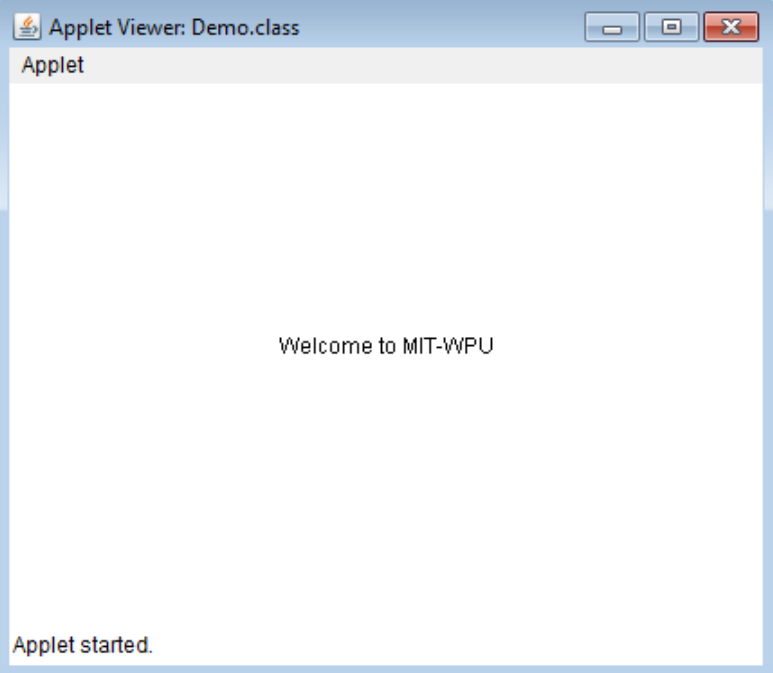
\includegraphics[scale=0.4]{../Programs/java_implementations/assignment_9/output_assignment_9.png}
\end{figure}


\section{Conclusion}
Thus, learned to use polymorphism and implemented solution of the given problem statement using C++ and Java.
\pagebreak

\section{FAQs}

\begin{enumerate}
	\item \textbf{Why do we use Exception Handling mechanism?}\\
	      Exception handling is the process of responding to unwanted or unexpected events when a computer program runs. Exception handling deals with these events to avoid the program or system crashing, and without this process, exceptions would disrupt the normal operation of a program.
	      \begin{enumerate}
		      \item It helps you avoid the program from crashing
		      \item It helps you set the program control in a more detailed manner
		      \item It helps you manually stop the program safely according to your wish.
	      \end{enumerate}
	      \begin{verbatim}
		// Psudo code for exception handling
		int a;
		try
		{
			cin>> a;
			cout<<33/a; // if a is 0, Exception is thrown, program crashes. 
		}
		catch DivisionByZeroException as e
		{
			cout<<"cant divide by zero;
		}
	\end{verbatim}
	\item \textbf{Is it possible to use multiple catch for single throw? Explain?}\\
	      Yes, it is possible to use multiple catch statements for a single throw statement in both C++ and Java. C++ try and catch block works in a specific way, where the throw keyword throws an exception with an integer, or an exception. You can then write multiple catch statements just below the try block.\\
	      In Java, you can throw instances of the Exception class, or throw any of the pre defined exceptions in java.

	      \textbf{Example}
	      \begin{lstlisting}[language=C++]
		int a;
		try
		{
			cin>> a;
			if(a == 0)
			{
				throw a; // int is being thrown. 
			}
			else{
				cout<<33/a; 
				throw 'a'; // character is being thrown.  
			}
		}
		catch (int a)
		{
			cout<<"cant divide by zero;
		}
		catch (char a)
		{
			cout<<"A is not zero";
		}
	\end{lstlisting}
	      \begin{lstlisting}[language = Java]
		try {
            withdrawal_amt = input.nextInt();
            if (withdrawal_amt > amount) {
                throw new Exception("Withdrawal amount more than amount. ");
				new_amount = withdrawal_amt / amount;
            } else {
                amount -= withdrawal_amt;
            }
        } catch (Exception e) {
            System.out.println("Withdrawal Amount more than amount in bank. ");
            return 0;
        } catch (DivisionByZeroException d)
		{
			System.out.println(d);
		}
	\end{lstlisting}
	\item \textbf{What is Exception Specification?}\\
	      An exception specification is a contract between the function and the rest of the program. It is a guarantee that the function will not throw any exception not listed in its exception specification.
	      \begin{lstlisting}[language = C++]
		void f1(void) throw(int) {   
			printf_s("About to throw 1\n");   
			if (1)   
			   throw 1;   
		 }   
	\end{lstlisting}
	      \begin{lstlisting}[language=Java]
		void function_name() throw(Exception)
		{
		  if (error) 
		  {
			throw Exception("Error");
		  }
		}		
	\end{lstlisting}
	\item \textbf{What is Re-throwing Exception?}\\
	      If a catch block cannot handle the exception that it was designed to handle, then you can rethrow that exception from that catch block.
	      It causes the original exception to be rethrown.

	      Because the exception has already been caught at the scope in which the rethrow expression occurs, it is rethrown out to the next dynamically enclosing try block. Therefore, it cannot be handled by catch blocks at the scope in which the rethrow expression occurred. Any catch blocks for the dynamically enclosing try block have an opportunity to catch the exception.
	      \begin{lstlisting}[language=C++]
		void f() {
			try {
			  cout << "In try block of f()" << endl;
			  cout << "Throwing exception of type E1" << endl;
			  E1 myException;
			  throw myException;
			}
			catch (E2& e) {
			  cout << "In handler of f(), catch (E2& e)" << endl;
			  cout << "Exception: " << e.message << endl;
			  throw;
			}
			catch (E1& e) {
			  cout << "In handler of f(), catch (E1& e)" << endl;
			  cout << "Exception: " << e.message << endl;
			  throw;
			}	
		}
		
	\end{lstlisting}
	\item \textbf{Explain use of finally keyword in java.}\\
	      Java finally block is a block used to execute important code such as closing the connection, etc.

	      Java finally block is always executed whether an exception is handled or not. Therefore, it contains all the necessary statements that need to be printed regardless of the exception occurs or not.

	      The finally block follows the try-catch block.

	      \begin{lstlisting}[language=Java]
	class TestFinallyBlock {    
		public static void main(String args[]){    
		try{    
	  //below code do not throw any exception  
		 int data=25/5;    
		 System.out.println(data);    
		}    
	  //catch won't be executed  
		catch(NullPointerException e){  
	  System.out.println(e);  
	  }    
	  //executed regardless of exception occurred or not  
	   finally {  
	  System.out.println("finally block is always executed");  
	  }    
\end{lstlisting}
\end{enumerate}

\end{document}